%%%%%%%%%%%%%%%%%%%%%%%%%%%%%%%%%%%%%%%%%%%%%%%%%%%%%%%%%%%%%%%%%%%%%%%%%%%%%%%%
% ACM Submission: Ownership Verification for Diffusion Models
% via T-Error and Gaussian Quantile Regression
%
% Converted from ICML 2026 format to acmart sigconf.
%%%%%%%%%%%%%%%%%%%%%%%%%%%%%%%%%%%%%%%%%%%%%%%%%%%%%%%%%%%%%%%%%%%%%%%%%%%%%%%%

\documentclass[sigconf, review, anonymous]{acmart}

%% ---- Placeholder rights metadata (fill in after venue acceptance) ----
\setcopyright{none}
\copyrightyear{2026}
\acmYear{2026}
\acmDOI{XXXXXXX.XXXXXXX}
\acmConference[Conference '26]{ACM Conference (placeholder)}{Month DD--DD, 2026}{City, Country}
\acmISBN{978-1-4503-XXXX-X/2026/XX}

%% ---- Packages (safe to use with acmart) ----
%% Note: booktabs, graphicx, natbib, hyperref, xcolor, amsmath are auto-loaded.
\usepackage{subcaption}
\usepackage{multirow}
\usepackage{xspace}
\usepackage{pifont}
\newcommand{\cmark}{\ding{51}}
\newcommand{\xmark}{\ding{55}}

%% ---- TikZ ----
\usepackage{tikz}
\usetikzlibrary{positioning,arrows.meta,calc,fit,shapes.geometric}

%% ---- Algorithms (not auto-loaded by acmart) ----
\usepackage{algorithm}
\usepackage{algorithmic}

%% ---- Custom commands ----
\newcommand{\terr}{\ensuremath{e_t}\xspace}
\newcommand{\Wset}{\ensuremath{\mathcal{W}}\xspace}
\newcommand{\Dtrain}{\ensuremath{\mathcal{D}_{\text{train}}}\xspace}
\newcommand{\Dpublic}{\ensuremath{\mathcal{D}_{\text{public}}}\xspace}
\newcommand{\MIA}{\textsc{MIA}\xspace}
\newcommand{\OV}{\textsc{OV}\xspace}

%% ---- Theorem environments ----
%% acmart defines: theorem, conjecture, proposition, lemma, corollary, example, definition
%% We only need to add 'claim' (not built-in).
\newtheorem{claim}{Claim}

%% =====================================================================
\begin{document}

\title[Membership is Ownership]{Membership is Ownership: A Robust Model Watermark Detection with Quantile Regression}

%% ---- Authors (anonymized during review) ----
\author{Feng Jiang}
\email{fjiang4@student.gsu.edu}
\affiliation{%
  \institution{Georgia State University}
  \city{Atlanta}
  \state{Georgia}
  \country{USA}}

\author{Zuobin Xiong}
\email{zxiong2@student.gsu.edu}
\affiliation{%
  \institution{Georgia State University}
  \city{Atlanta}
  \state{Georgia}
  \country{USA}}

\author{An Huang}
\email{ahuang8@student.gsu.edu}
\affiliation{%
  \institution{Georgia State University}
  \city{Atlanta}
  \state{Georgia}
  \country{USA}}

\author{Zhipeng Cai}
\email{zcai@gsu.edu}
\affiliation{%
  \institution{Georgia State University}
  \city{Atlanta}
  \state{Georgia}
  \country{USA}}

\author{Yingshu Li}
\email{yli@gsu.edu}
\affiliation{%
  \institution{Georgia State University}
  \city{Atlanta}
  \state{Georgia}
  \country{USA}}

\renewcommand{\shortauthors}{Jiang et al.}

%% ---- Abstract (must appear before \maketitle in acmart) ----
\begin{abstract}
Large-scale diffusion models are valuable intellectual property, yet can be stolen and adapted via downstream fine-tuning.
Existing diffusion watermarking embeds explicit signatures into parameters or behavior, which may degrade utility and can be removed by post-hoc fine-tuning.
We propose {Membership Is Ownership}, an ownership verification framework that treats a private member evidence set as a watermark and leverages the model's intrinsic memorization.
Given a suspect model, we compute a multi-timestep \emph{t-error} score by forward noising and single-step reconstruction, then aggregate with a lower quantile (Q25).
To control false-positive rates, we fit a conditional Gaussian model in log-score space and obtain closed-form quantile thresholds at arbitrary target FPR.
The protocol compares the suspect model against public baselines via hypothesis tests, effect sizes, and error ratios, producing statistical evidence rather than a single score.
On CIFAR-10/100, STL-10, and CelebA, all datasets achieve Cohen's $d > 18$ and error ratios $> 19\times$ against public baselines; these separations persist after MMD fine-tuning (simulating post-theft adaptation), provided the adversary does not retrain from scratch.
\end{abstract}

%% ---- CCS Concepts (placeholder — generate at https://dl.acm.org/ccs/ccs.cfm) ----
\begin{CCSXML}
<ccs2012>
 <concept>
  <concept_id>10010147.10010257.10010293.10010294</concept_id>
  <concept_desc>Computing methodologies~Neural networks</concept_desc>
  <concept_significance>500</concept_significance>
 </concept>
 <concept>
  <concept_id>10002978.10002991.10002992</concept_id>
  <concept_desc>Security and privacy~Digital rights management</concept_desc>
  <concept_significance>500</concept_significance>
 </concept>
 <concept>
  <concept_id>10002978.10003006.10003007</concept_id>
  <concept_desc>Security and privacy~Watermarking</concept_desc>
  <concept_significance>300</concept_significance>
 </concept>
</ccs2012>
\end{CCSXML}
\ccsdesc[500]{Computing methodologies~Neural networks}
\ccsdesc[500]{Security and privacy~Digital rights management}
\ccsdesc[300]{Security and privacy~Watermarking}

\keywords{diffusion models, ownership verification, watermarking, membership inference, quantile regression}

\maketitle

%%%%%%%%%%%%%%%%%%%%%%%%%%%%%%%%%%%%%%%%%%%%%%%%%%%%%%%%%%%%%%%%%%%%%%%%%%%%%%%%
% 1. INTRODUCTION
%%%%%%%%%%%%%%%%%%%%%%%%%%%%%%%%%%%%%%%%%%%%%%%%%%%%%%%%%%%%%%%%%%%%%%%%%%%%%%%%
\section{Introduction}
\label{sec:intro}

Large-scale generative diffusion models have fueled numerous profitable downstream applications.
To obtain such powerful models, a huge amount of computation and data resources are consumed, which renders the trained diffusion models valuable intellectual property (IP) for tech companies and individuals.
However, these IP assets are vulnerable to various unauthorized uses by adversaries seeking to leverage these models for customized, usually commercial applications.

In practice, an adversary can obtain a checkpoint via model extraction attacks or illicit transfer, then fine-tune the model to a profitable domain or product requirement~\cite{wang2025sleepermark,kim2024wouaf}.
Such post-theft fine-tuning undermines the model owner's copyright and poses significant challenges for reliable ownership verification.
To make a strong claim, the owner must produce evidence that is not only accurate under stringent false-positive budgets,
and also valid after realistic fine-tune or adaptation.

Most existing diffusion IP protection methods embed explicit signatures into model parameters or output behavior~\citep{peng2023watermark,zhao2023recipe,fernandez2023stable,liu2023watermarking}.
While effective in controlled settings, such watermarks may impose utility costs and can be weakened by fine-tuning because the model thief can use every means to remove such explicit watermarks.
Recently, an alternative watermark method has emerged, which is to leverage the model's intrinsic memorization~\citep{carlini2023extracting,somepalli2023diffusion,gu2025on} , where the reconstruction error of diffusion models on training examples is systematically lower than on non-training samples.
However, as the models' generalization capability increases, the difference between training samples and non-training samples becomes marginal, resulting in the ``low error-based'' method being insufficient for an ownership claim.
Moreover, most modern diffusion models may also use substantially overlapped training data from the public Internet, which increases the difficulty of accurate attribution.

These practical challenges necessitate a robust watermark detection method that can distinguish the IP-protected model from public reference models under a statistically controlled decision rule.
To fill this research gap, in this work, we propose \textbf{Membership is Ownership}, an ownership verification framework that can accurately detect and verify whether a suspect model in the thief's possession is illegally obtained and fine-tuned from the model owner's base model, using a designated owner signature.
At the heart of our approach lies a simple but principled observation: a model retains systematic memory of its training data, manifesting as lower reconstruction error on seen examples. We exploit this signal by constructing a private evidence set, cryptographically signed by the model owner, which serves as a persistent watermark without modifying the model itself.
To extract a robust signal from a suspect model, we introduce a multi-timestep \emph{t-error} score—computed via forward noising followed by single-step reconstruction—and summarize it through a lower quantile (\texttt{Q25}) to suppress noise while preserving the memorization signature. Rather than reporting a single black-box decision, we anchor the verification protocol on a principled statistical foundation: a conditional Gaussian model fitted in log-score space yields closed-form quantile thresholds at arbitrary false-positive rates, enabling transparent and auditable comparisons against public baselines through hypothesis tests, effect sizes, and error ratios.
The resulting separations are striking. Against public baselines, we observe Cohen's $d > 18$ and error ratios exceeding $19\times$, margins that remain robust even under MMD fine-tuning, which simulates realistic post-theft adaptation, provided the adversary stops short of full retraining or targeted memorization erasure.
The paper unfolds the following contributions.
\begin{itemize}
    \item We introduce a training-free ownership verification framework
    for diffusion models that leaves model parameters and output
    quality entirely intact, relying solely on a private evidence
    set as a non-invasive watermark.

    \item We propose a multi-timestep $t$-error score aggregated via
    lower quantile (\texttt{Q25}), which suppresses per-example noise
    while preserving the memorization signal, yielding a stable and
    discriminative per-sample statistic.

    \item We derive closed-form quantile thresholds under a conditional
    Gaussian model in log-score space, enabling precise false-positive
    rate control at any target significance level without requiring
    empirical calibration.

    \item We demonstrate Cohen's $d > 18$ and error ratios exceeding
    $19\times$ across four datasets, with separations remaining robust
    under MMD fine-tuning, establishing strong empirical guarantees
    against realistic post-theft adaptation.
\end{itemize}


\begin{figure*}[t]
\centering
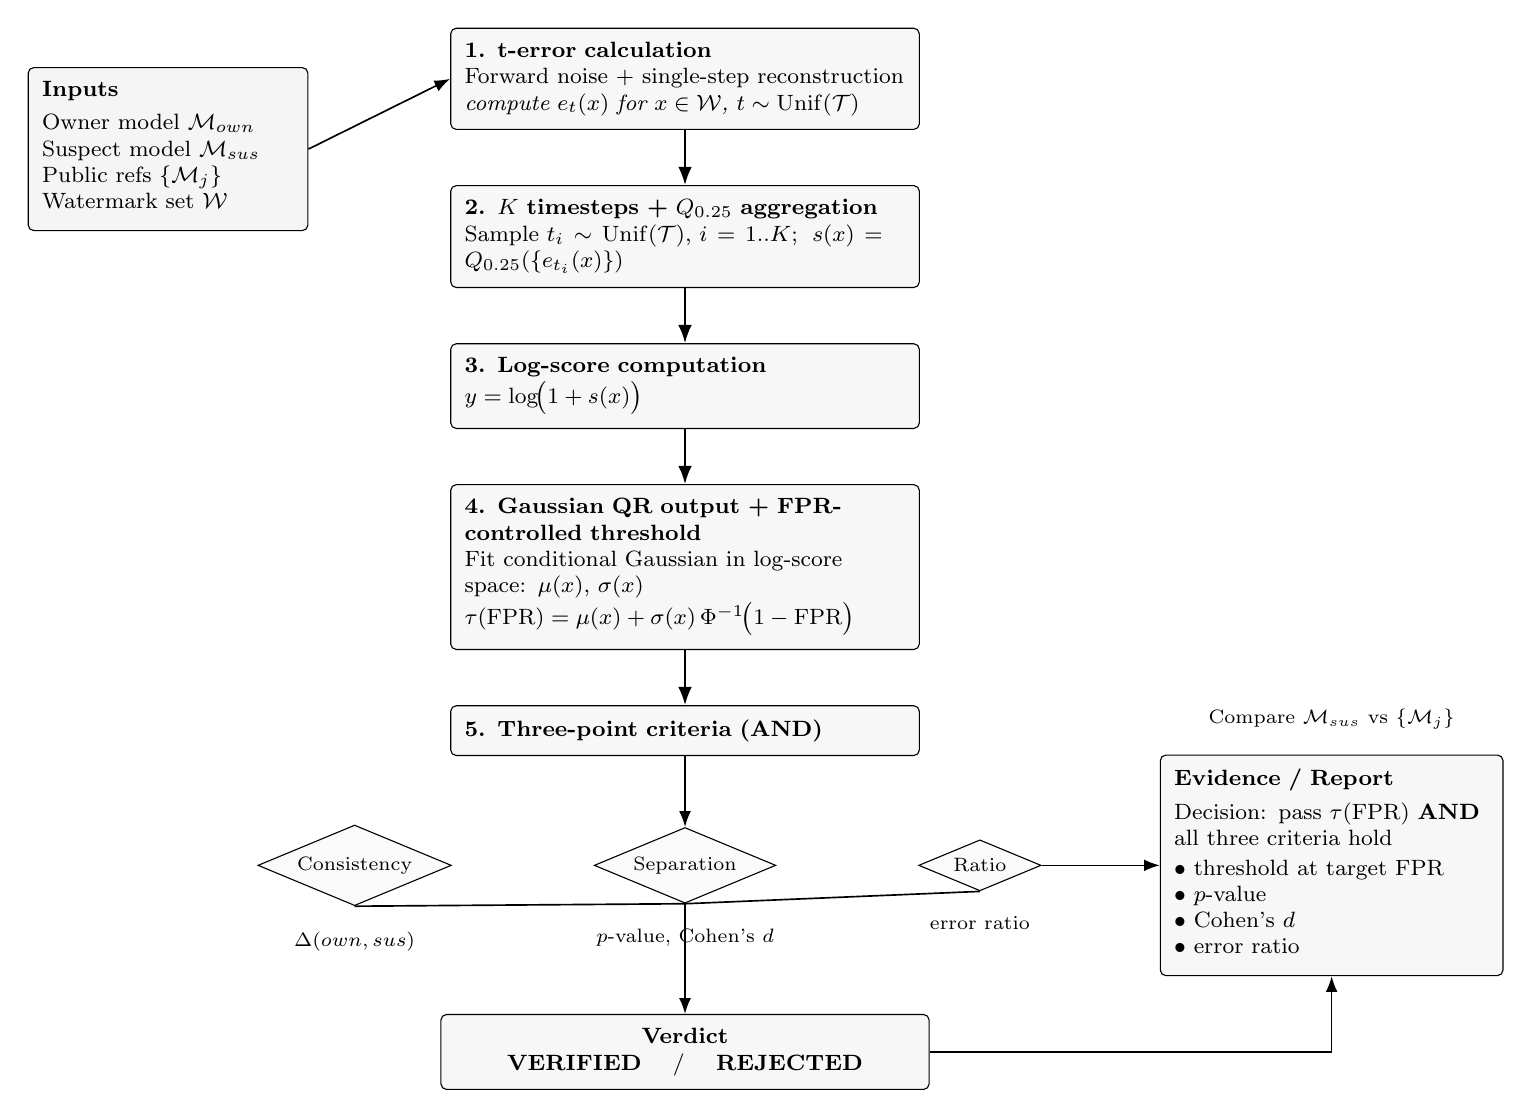
\begin{tikzpicture}[
  font=\footnotesize,
  line/.style={-Latex, thick, draw=black},
  thinline/.style={-Latex, semithick, draw=black},
  box/.style={draw=black, rounded corners=2pt, align=left, inner sep=5pt, fill=gray!8, text width=3.2cm},
  stepbox/.style={draw=black, rounded corners=2pt, align=left, inner sep=5pt, fill=gray!6, text width=5.6cm},
  outbox/.style={draw=black, rounded corners=2pt, align=left, inner sep=5pt, fill=gray!6, text width=4.0cm},
  diamondbox/.style={draw=black, diamond, aspect=2.4, inner sep=2pt, fill=gray!4, font=\scriptsize},
  decision/.style={draw=black, rounded corners=2pt, align=center, inner sep=5pt, fill=gray!6, text width=5.2cm},
  notelabel/.style={font=\scriptsize, text=black}
]

% ========== LEFT: Inputs ==========
\node[box] (inputs) at (0,0) {%
\textbf{Inputs}\vspace{1mm}\par
\begin{tabular}{@{}l@{}}
Owner model $\mathcal{M}_{\text{own}}$\\
Suspect model $\mathcal{M}_{\text{sus}}$\\
Public refs $\{\mathcal{M}_j\}$\\
Watermark set $\mathcal{W}$\\
\end{tabular}
};

% ========== CENTER: Pipeline (5 steps, vertical) ==========
\node[stepbox, right=18mm of inputs.north east, anchor=north west, yshift=5mm] (s1)
{\textbf{1. t-error calculation}\par
Forward noise + single-step reconstruction\par
\emph{compute $e_t(x)$ for $x\in\mathcal{W}$, $t\sim\mathrm{Unif}(\mathcal{T})$}
};

\node[stepbox, below=7mm of s1] (s2)
{\textbf{2. $K$ timesteps + $Q_{0.25}$ aggregation}\par
Sample $t_i\sim \mathrm{Unif}(\mathcal{T}),\, i=1..K$;\;
$s(x)=Q_{0.25}\!\left(\{e_{t_i}(x)\}\right)$
};

\node[stepbox, below=7mm of s2] (s3)
{\textbf{3. Log-score computation}\par
$y=\log\!\bigl(1+s(x)\bigr)$
};

\node[stepbox, below=7mm of s3] (s4)
{\textbf{4. Gaussian QR output + FPR-controlled threshold}\par
Fit conditional Gaussian in log-score space: $\mu(x),\,\sigma(x)$\par
$\tau(\mathrm{FPR})=\mu(x)+\sigma(x)\,\Phi^{-1}\!\bigl(1-\mathrm{FPR}\bigr)$
};

\node[stepbox, below=7mm of s4] (s5)
{\textbf{5. Three-point criteria (AND)}\par
};

% Criteria diamonds (c2 centered below s5 for vertical arrow)
\node[diamondbox, below=9mm of s5] (c2) {Separation};
\node[diamondbox, left=18mm of c2] (c1) {Consistency};
\node[diamondbox, right=18mm of c2] (c3) {Ratio};

\node[notelabel, below=2mm of c1] (lbl1) {$\Delta(\text{own},\text{sus})$};
\node[notelabel, below=2mm of c2] (lbl2) {$p$-value, Cohen's $d$};
\node[notelabel, below=2mm of c3] (lbl3) {error ratio};

% Decision box
\node[decision, below=14mm of c2, minimum width=62mm] (verdict)
{\textbf{Verdict}\par
\textbf{VERIFIED} \quad / \quad \textbf{REJECTED}
};

% -----------------------------
% Output / Evidence report (aligned with Ratio for horizontal arrow)
% -----------------------------
\node[outbox, right=15mm of c3.east, anchor=west] (report)
{\textbf{Evidence / Report}\vspace{1mm}\par
Decision: pass $\tau(\mathrm{FPR})$ \textbf{AND} all three criteria hold\par\vspace{1mm}
\begin{tabular}{@{}l@{}}
$\bullet$ threshold at target FPR\\
$\bullet$ $p$-value\\
$\bullet$ Cohen's $d$\\
$\bullet$ error ratio\\
\end{tabular}
};

% -----------------------------
% Arrows (orthogonal Manhattan routing)
% -----------------------------

% ===== P0-1: Inputs → Step1 (single horizontal arrow) =====
\draw[thinline] (inputs.east) -- (s1.west);

% ===== Pipeline arrows (vertical) =====
\draw[line] (s1) -- (s2);
\draw[line] (s2) -- (s3);
\draw[line] (s3) -- (s4);
\draw[line] (s4) -- (s5);

% ===== Step5 → Separation (pure vertical) =====
\draw[thinline] (s5.south) -- (c2.north);

% ===== Horizontal bus connecting diamonds =====
\draw[semithick] (c1.south) -- (c2.south) -- (c3.south);

% ===== Bus center → Verdict (vertical) =====
\draw[thinline] (c2.south) -- (verdict.north);

% ===== Ratio → Evidence (pure horizontal) =====
\draw[thinline] (c3.east) -- (report.west);

% ===== Verdict → Evidence (L-shape: horizontal right, then vertical up) =====
\draw[thinline] (verdict.east) -| (report.south);

% ===== Label above report =====
\node[notelabel, above=2mm of report] {Compare $\mathcal{M}_{\text{sus}}$ vs $\{\mathcal{M}_j\}$};

\end{tikzpicture}
\caption{\textbf{System overview.}
A private evidence set $\mathcal{W}$ serves as a watermark. We compute multi-timestep t-error scores, aggregate with a robust lower quantile to obtain $s(x)$, and fit a conditional Gaussian model in log-score space to derive a closed-form threshold at a target FPR. Ownership is supported via population-level evidence against public reference models using consistency, separation, and ratio criteria.}
\Description{A flowchart showing the MiO ownership verification pipeline. From left to right: inputs (owner model, suspect model, public references, watermark set) feed into a five-step vertical pipeline (t-error calculation, K-timestep Q25 aggregation, log-score computation, Gaussian QR threshold, three-point criteria). Three diamond decision nodes (consistency, separation, ratio) lead to a verdict (verified or rejected) and an evidence report listing the threshold, p-value, Cohen's d, and error ratio.}
\label{fig:overview}
\end{figure*}

%%%%%%%%%%%%%%%%%%%%%%%%%%%%%%%%%%%%%%%%%%%%%%%%%%%%%%%%%%%%%%%%%%%%%%%%%%%%%%%%
% 2. RELATED WORK
%%%%%%%%%%%%%%%%%%%%%%%%%%%%%%%%%%%%%%%%%%%%%%%%%%%%%%%%%%%%%%%%%%%%%%%%%%%%%%%%
\section{Related Work}
\label{sec:related}

\paragraph{Model Watermarking.}
Prior machine learning model watermarking methods typically embed an identifiable pattern into model behavior, most notably through trigger-based backdoors or carefully constructed inputs that induce a predetermined response~\citep{adi2018turning,zhang2018protecting,fernandez2023stable,wen2023tree}.
Such approaches provide a direct verification interface when the watermark remains intact, but they generally require explicit intervention during training and can be sensitive to subsequent model editing or ``cleaning.''
\textit{In contrast to embedding an external trigger, our setting treats a private member evidence set as the ``watermark'' and derives evidence from the model's intrinsic memorization behavior, avoiding modifications that introduce new behavioral artifacts.}

\paragraph{Membership Inference Attacks.}
Membership inference attacks (MIA) aim to decide whether an input was part of a model's training data~\citep{shokri2017membership,yeom2018privacy,salem2019ml}.
For diffusion models, recent work instantiates MIA using reconstruction-based signals~\citep{carlini2023extracting,duan2023diffusion,kong2024efficient}, loss/likelihood-based criteria~\citep{matsumoto2023membership,hu2023loss}, or scalable quantile-regression formulations~\citep{bertran2023scalable,tang2024membership}.
These methods are primarily evaluated as per-example decision rules (binary classification or scoring) and are typically reported via attack metrics.
Ownership verification, however, requires comparative, population-level evidence: the ownership claim must be supported by aggregate separation on a designated evidence set, calibrated against reference models that represent the null hypothesis, and summarized via statistically interpretable tests rather than single-sample predictions.
\textit{Our framework uses MIA-style signals as the underlying measurements, but creates an auditable verification procedure with public references and formal decision criteria.}
%%%%%%%%%%%%%%%%%%%%%%%%%%%%%%%%%%%%%%%%%%%%%%%%%%%%%%%%%%%%%%%%%%%%%%%%%%%%%%%%
% 3. PROBLEM SETUP
%%%%%%%%%%%%%%%%%%%%%%%%%%%%%%%%%%%%%%%%%%%%%%%%%%%%%%%%%%%%%%%%%%%%%%%%%%%%%%%%
\section{Problem Setup}
\label{sec:problem}

\subsection{Background and Problem Formulation }

\paragraph{Diffusion Models.}
A diffusion model defines a forward noising process and a learned
reverse process. Given a clean sample $x_0 \sim q(x_0)$, the
forward process produces a noisy version at timestep $t \in
\{1, \dots, T\}$:
%
\begin{equation}
    x_t = \sqrt{\bar\alpha_t}\, x_0
        + \sqrt{1 - \bar\alpha_t}\,\epsilon,
    \quad \epsilon \sim \mathcal{N}(0, I),
\end{equation}
%
where $\bar\alpha_t = \prod_{s=1}^{t} \alpha_s$ is the cumulative
noise schedule. A neural network $\epsilon_\theta$ is trained to
recover the added noise by minimizing:
%
\begin{equation}
    \mathcal{L}(\theta)
    = \mathbb{E}_{x_0,\, \epsilon,\, t}
      \bigl[\lVert \epsilon
      - \epsilon_\theta(x_t, t) \rVert^2\bigr].
\end{equation}
%
At inference, new samples are drawn by iteratively denoising from
$x_T \sim \mathcal{N}(0, I)$ using the learned
$\epsilon_\theta$.

It has been empirically established that diffusion models memorize
portions of their training data~\cite{carlini2023extracting,
somepalli2023diffusion}: the reconstruction error on training
examples is systematically lower than on unseen samples drawn from
the same distribution. This memorization gap persists across
architectures and dataset scales, and serves as the foundational
signal that our framework exploits for ownership verification.

\paragraph{From Membership Inference to Ownership Verification.}
Membership inference attacks (MIAs) leverage the memorization gap
to determine whether a single query sample belongs to the training
set of a target model~\cite{duan2023diffusion, kong2024efficient}.
We state this formally:

\begin{definition}[Membership Inference Attack]
Given a target model $M$ and a query sample $x$, a
membership inference attack is a binary classifier
$\mathcal{A}: (M, x) \rightarrow \{0, 1\}$ that predicts
whether $x \in \mathcal{D}_{\mathrm{train}}$.
\end{definition}

However, low reconstruction error on a single sample does not constitute evidence of ownership, as the sample may simply be inherently easy to reconstruct for any model. Ownership
verification demands a stronger, population-level claim: the
suspect model must exhibit statistically significant memorization
on a \emph{designated evidence set} when compared against public
baselines that share no training overlap with that set.

\begin{definition}[Ownership Verification]
Let $\mathcal{M}_A$ denote a base model trained by the
owner, $\mathcal{M}_B$ a suspect model held by the
adversary, and $\mathcal{W} = \{x_1, \dots, x_{|\mathcal{W}|}\}$ a private
evidence set signed by the owner such that
$\mathcal{W} \subset \mathcal{D}_{\mathrm{train}}
(\mathcal{M}_A)$. An ownership verification protocol is
a hypothesis test
$\mathcal{V}: (\mathcal{M}_B, \mathcal{W},
\{M_{\text{ref}}^{(i)}\}) \rightarrow
\{\texttt{owned}, \texttt{independent}\}$
that determines whether $\mathcal{M}_B$ is derived from
$\mathcal{M}_A$ by comparing the reconstruction behavior
of $\mathcal{M}_B$ on $\mathcal{W}$ against a set of
public baseline models
$\{M_{\text{ref}}^{(i)}\}_{|\mathcal{T}|=1}^{|\mathcal{T}|}$ at a controlled
false-positive rate $\alpha$.
\end{definition}

This formulation shifts the task from sample-level binary
classification to a calibrated, population-level statistical test,
which is the protocol we develop in the following sections.

\subsection{Threat Model}

We consider three principals in the ownership verification setting.
The \textbf{owner} $O$ trains a model $\mathcal{M}_A$ on
$\mathcal{D}_{\mathrm{train}}$, which contains a private watermark
set $\mathcal{W} \subset \mathcal{D}_{\mathrm{train}}$ known only
to $O$.
The \textbf{adversary} obtains $\mathcal{M}_A$ through theft or
leakage, and produces a derivative model $\mathcal{M}_B$ by
fine-tuning; $\mathcal{M}_B$ is the suspect model submitted for
verification.
The \textbf{verifier} $V$, given $\mathcal{M}_A$, $\mathcal{M}_B$,
a set of public baseline models, and the private set $\mathcal{W}$,
determines whether the ownership claim is valid.

We assume the adversary has white-box access to $\mathcal{M}_A$
and may possess in-domain data disjoint from $\mathcal{W}$. The
adversary is aware that a verification protocol exists but cannot
identify $\mathcal{W}$: beyond the owner's secrecy, even if
$\mathcal{D}_{\mathrm{train}}$ were leaked, selecting the exact
$|\mathcal{W}|$-subset from $N$ training samples is feasible with probability
at most
%
\begin{equation}
    P(\text{exact match})
    = \frac{1}{\binom{N}{|\mathcal{W}|}}
    \;\leq\; \left(\frac{|\mathcal{W}|}{N}\right)^{|\mathcal{W}|},
\end{equation}
%
which evaluates to $10^{-5000}$ under the CIFAR-10 setting
($N=50{,}000$, $|\mathcal{W}|=5{,}000$), making exhaustive guessing
computationally infeasible. This bound rests on a counting
argument rather than a cryptographic assumption and does not
claim resistance to side-channel leakage of $\mathcal{W}$ itself.
The adversary is permitted to apply fine-tuning, distillation,
and pruning to $\mathcal{M}_A$; full retraining from scratch
falls outside our scope, as it severs provenance entirely.

Upon receiving a dispute, the verifier proceeds as follows:
it first checks that $\mathrm{SHA\text{-}256}(\mathrm{sort}
(\mathcal{W}))$ matches a hash commitment timestamped prior to
the dispute; it then computes $t$-error scores on $\mathcal{W}$ for both the suspect model and public baselines; and finally
evaluates the three-point criteria (Section~\ref{sec:criteria}),
outputting \textsc{Verified} or \textsc{Rejected} together with
the supporting statistical evidence ($p$-values, Cohen's $d$,
and error ratio). The verifier is assumed to have white-box
access to both models, consistent with standard practice in IP
litigation, regulatory audits, and contractual audit clauses.
%%%%%%%%%%%%%%%%%%%%%%%%%%%%%%%%%%%%%%%%%%%%%%%%%%%%%%%%%%%%%%%%%%%%%%%%%%%%%%%%
% 4. METHOD
%%%%%%%%%%%%%%%%%%%%%%%%%%%%%%%%%%%%%%%%%%%%%%%%%%%%%%%%%%%%%%%%%%%%%%%%%%%%%%%%
\section{Method}
\label{sec:method}

The verification framework has four components:
(1) a \emph{t-error} score measuring reconstruction quality via forward-reverse diffusion,
(2) multi-timestep aggregation for stable per-sample scores, (3) Gaussian quantile regression for FPR-controlled thresholds,
and (4) a three-point statistical protocol comparing the suspect model against public baselines.

\subsection{$t$-error Scoring}
\label{sec:t_error}

Diffusion models reconstruct their training data with lower error than unseen data~\citep{carlini2023extracting}. We exploit this \emph{memorization gap} by measuring reconstruction quality at a given noise level $t$.

Specifically, given a clean sample $x_0$, we first corrupt it via the forward diffusion schedule:
\begin{equation}
x_t = \sqrt{\bar{\alpha}_t} \cdot x_0 + \sqrt{1 - \bar{\alpha}_t} \cdot \epsilon, \quad \epsilon \sim \mathcal{N}(0, I)
\end{equation}
where $x_t$ is the noised image at timestep $t \in \{1,\ldots,T\}$, $\epsilon$ is i.i.d.\ Gaussian noise, and $\bar{\alpha}_t = \prod_{s=1}^{t} \alpha_s$ is the cumulative noise coefficient under a cosine schedule~\citep{dhariwal2021diffusion}. The model then predicts the added noise $\hat{\epsilon}_\theta(x_t, t)$, from which we recover a single-step reconstruction:
\begin{equation}
\hat{x}_0 = \frac{x_t - \sqrt{1 - \bar{\alpha}_t} \cdot \hat{\epsilon}_\theta(x_t, t)}{\sqrt{\bar{\alpha}_t}}
\end{equation}
We define the \emph{$t$-error}, denoted $e_t(x_0)$, as the per-pixel mean squared error between the original and reconstructed images:
\begin{equation}
e_t(x_0) = \frac{\|x_0 - \hat{x}_0\|_2^2}{H \times W \times C}
\end{equation}
where $H$, $W$, $C$ denote the image height, width, and number of channels, respectively. The key property underlying our framework is the \emph{memorization effect}: models trained on a particular dataset exhibit systematically lower reconstruction error on their training examples, i.e., $\mathbb{E}_{x \in \mathcal{D}_{\mathrm{train}}}[e_t(x)] < \mathbb{E}_{x \notin \mathcal{D}_{\mathrm{train}}}[e_t(x)]$. This persistent gap, which survives across architectures and dataset scales, provides the foundational signal for our ownership verification protocol.

\subsection{Multi-Timestep Aggregation}
\label{sec:aggregation}

A single timestep provides a noisy estimate of reconstruction quality, as the magnitude of $e_t(x)$ varies substantially with the noise level $t$. To obtain a stable per-sample statistic, we aggregate $t$-errors over $K$ uniformly sampled timesteps into a single score $s(x)$ via the 25th percentile:
\begin{equation}
  s(x) = Q_{0.25}\!\bigl(\{e_{t_i}(x)\}_{i=1}^{K}\bigr)
\end{equation}
We use $K{=}50$ by default. The choice of a lower percentile is deliberate: it captures the timesteps where the memorization gap is most pronounced while remaining robust to outlier timesteps that introduce high but uninformative error. Ablations in Section~\ref{sec:ablation} confirm that the 25th percentile yields the strongest separation among common aggregation strategies, and that performance is stable for $K \geq 25$. The full scoring procedure is summarized in Algorithm~\ref{alg:t_error}.

\begin{algorithm}[t]
\caption{$t$-error Computation}
\label{alg:t_error}
\begin{algorithmic}
\REQUIRE Model $\mathcal{M}$, sample $x_0$, timesteps $\mathcal{T} = \{t_1, \ldots, t_K\}$, noise schedule $\{\bar{\alpha}_t\}$
\ENSURE Aggregated score $s(x_0)$
\STATE $\texttt{errors} \leftarrow []$
\FOR{$t \in \mathcal{T}$}
    \STATE $\epsilon \sim \mathcal{N}(0, I)$
    \STATE $x_t \leftarrow \sqrt{\bar{\alpha}_t} \cdot x_0 + \sqrt{1 - \bar{\alpha}_t} \cdot \epsilon$
    \STATE $\hat{\epsilon} \leftarrow M_\theta(x_t, t)$
    \STATE $\hat{x}_0 \leftarrow (x_t - \sqrt{1 - \bar{\alpha}_t} \cdot \hat{\epsilon}) / \sqrt{\bar{\alpha}_t}$
    \STATE $e_t \leftarrow \|x_0 - \hat{x}_0\|_2^2 / (H \times W \times C)$
    \STATE $\texttt{errors}.\text{append}(e_t)$
\ENDFOR
\STATE \textbf{return} $s(x_0) \leftarrow Q_{0.25}(\texttt{errors})$
\end{algorithmic}
\end{algorithm}

\subsection{Gaussian Quantile Regression}
\label{sec:gaussian_qr}

Rather than relying on fixed thresholds, we model the \emph{conditional score distribution} for non-members and derive decision boundaries in closed form. Concretely, we apply a log transformation to the aggregated score and parameterize the result as a Gaussian with input-dependent mean $\mu(x)$ and standard deviation $\sigma(x)$:
\begin{equation}
y = \log(1 + s(x)) \sim \mathcal{N}\!\bigl(\mu(x),\, \sigma^2(x)\bigr)
\end{equation}
where $\mu(x)$ and $\sigma(x)$ are jointly predicted by a neural network $f_\psi$. The network uses a ResNet-18 backbone to extract image features, which are concatenated with a compact statistical summary $\phi(x) \in \mathbb{R}^3$ consisting of the mean, standard deviation, and $\ell_2$ norm of the $t$-error sequence. An MLP head maps the combined representation to $(\mu, \log\sigma)$.

We train $f_\psi$ by minimizing the Gaussian negative log-likelihood over $N$ auxiliary non-member samples:
\begin{equation}
\mathcal{L}_{\text{NLL}} = \frac{1}{N}\sum_{i=1}^{N}\left[\frac{(y_i - \mu_i)^2}{2\sigma_i^2} + \log\sigma_i\right]
\end{equation}
where $y_i = \log(1 + s(x_i))$ is the observed log-score and $(\mu_i, \sigma_i)$ are the corresponding network predictions. Because the conditional distribution is Gaussian, the $(1{-}\alpha)$-quantile at any target false-positive rate $\alpha$ admits a closed-form expression:
\begin{equation}
\hat{q}_\tau(x) = \mu(x) + \sigma(x) \cdot \Phi^{-1}(\tau), \quad \tau = 1 - \alpha
\end{equation}
with $\Phi^{-1}$ denoting the standard normal inverse CDF. This is a key practical advantage over pinball-loss quantile regression, which requires training a separate model for every desired quantile level; here, a single model supports arbitrary $\tau$ without retraining.

To translate the predicted quantile into a membership decision, we define the \emph{margin} $m_\tau(x)$ as the gap between the predicted quantile and the observed log-score:
\begin{equation}
m_\tau(x) = \hat{q}_\tau(x) - \log(1 + s(x))
\end{equation}
A positive margin indicates that the sample's reconstruction error falls below what would be expected of a non-member, suggesting likely membership in the training set.

Finally, to reduce prediction variance, we wrap the above procedure in a bagging ensemble of $B{=}50$ models, each trained on a bootstrap sample drawn with replacement from 80\% of the auxiliary data. At inference, we average the individual quantile predictions into a single ensemble estimate:
\begin{equation}
\hat{q}_\tau^{\text{ens}}(x) = \frac{1}{B}\sum_{b=1}^{B}\hat{q}_\tau^{(b)}(x)
\end{equation}
where $\hat{q}_\tau^{(b)}(x)$ is the quantile from the $b$-th ensemble member. The ensemble margin $m_\tau^{\text{ens}}(x) = \hat{q}_\tau^{\text{ens}}(x) - \log(1 + s(x))$ serves as the final per-sample statistic; as before, positive values indicate likely membership. Ensembling is embarrassingly parallel and introduces negligible additional inference cost (Section~\ref{sec:cost}).

\subsection{Three-Point Verification Criteria}
\label{sec:criteria}

Given the owner model $\mathcal{M}_A$, the suspect model $\mathcal{M}_B$, a set of public baselines, and the watermark set $\Wset$, we require all three of the following criteria to be satisfied before declaring ownership verified.

\paragraph{Criterion 1: Consistency.}
If $\mathcal{M}_B$ is indeed derived from $\mathcal{M}_A$, the two models should exhibit similar reconstruction behavior on $\Wset$. We operationalize this by requiring that a two-sample $t$-test on their score distributions yields $p > 0.05$, i.e., we cannot reject the null hypothesis that the two models share the same $t$-error distribution. Failure here suggests that the suspect model has no provenance relationship with the owner model.

\paragraph{Criterion 2: Separation.}
The owner model must reconstruct watermark samples significantly better than any public baseline. We require both statistical significance ($p < 10^{-6}$, to control for multiple baseline comparisons) and practical significance (Cohen's $d > 2.0$, corresponding to a ``very large'' effect size~\citep{cohen1988statistical}). This dual requirement guards against claims that achieve a low $p$-value purely through large sample size without meaningful effect.

\paragraph{Criterion 3: Ratio.}
As a final, interpretable sanity check, we require the ratio of mean baseline score to mean owner score to exceed a conservative threshold:
\begin{equation}
\frac{\bar{s}_{\text{baseline}}}{\bar{s}_{\text{owner}}} > 5.0
\end{equation}
where $\bar{s}$ denotes the sample mean of aggregated $t$-error scores. This threshold is deliberately conservative; in all experiments the observed ratio exceeds $19\times$ (Table~\ref{tab:main_results}).

Ownership is declared \textbf{verified} only when all three criteria are jointly satisfied. This conjunction ensures that no single metric can produce a false positive: consistency confirms provenance, separation establishes that the memorization signal is genuine rather than coincidental, and the ratio provides a human-interpretable magnitude check. The complete verification protocol, including hash commitment validation, is formalized in Algorithm~\ref{alg:verification}.
\begin{algorithm}[t]
\caption{Ownership Verification Protocol}
\label{alg:verification}
\begin{algorithmic}
\REQUIRE Models $M_A, M_B$, baselines $\{M_{\text{ref}}^{(i)}\}$, watermark set $\mathcal{W}$, hash commitment $H_{\text{claimed}}$
\ENSURE $\textsc{Verified}$ or $\textsc{Rejected}$
\STATE $H_{\text{computed}} \leftarrow \text{SHA-256}(\text{sort}(\mathcal{W}))$
\IF{$H_{\text{computed}} \neq H_{\text{claimed}}$}
    \STATE \textbf{return} $\textsc{Rejected}$
\ENDIF
\STATE $S_A \leftarrow \{s_{M_A}(x) : x \in \mathcal{W}\}$; $S_B \leftarrow \{s_{M_B}(x) : x \in \mathcal{W}\}$
\STATE $S_{\text{ref}} \leftarrow \{s_{M_{\text{ref}}}(x) : x \in \mathcal{W}\}$ for best baseline
\STATE \textbf{O1:} $p_1 \leftarrow \text{TTest}(S_A, S_B)$; \textbf{if} $p_1 < 0.05$ \textbf{return} $\textsc{Rejected}$
\STATE \textbf{O2:} $p_2, d \leftarrow \text{TTest}(S_A, S_{\text{ref}}), \text{CohenD}(S_A, S_{\text{ref}})$
\IF{$p_2 > 10^{-6}$ \textbf{or} $|d| < 2.0$}
    \STATE \textbf{return} $\textsc{Rejected}$
\ENDIF
\STATE \textbf{O3:} $r \leftarrow \text{mean}(S_{\text{ref}}) / \text{mean}(S_A)$; \textbf{if} $r < 5.0$ \textbf{return} $\textsc{Rejected}$
\STATE \textbf{return} $\textsc{Verified}$
\end{algorithmic}
\end{algorithm}


%%%%%%%%%%%%%%%%%%%%%%%%%%%%%%%%%%%%%%%%%%%%%%%%%%%%%%%%%%%%%%%%%%%%%%%%%%%%%%%%
% 5. EXPERIMENTS
%%%%%%%%%%%%%%%%%%%%%%%%%%%%%%%%%%%%%%%%%%%%%%%%%%%%%%%%%%%%%%%%%%%%%%%%%%%%%%%%
\section{Experiments}
\label{sec:experiments}

\subsection{Experimental Setup}
\label{sec:setup}

We evaluate our framework on four datasets spanning different resolutions and scales: CIFAR-10 and CIFAR-100 (both 32$\times$32, 50k training images with 5k reserved as the watermark set), STL-10 (96$\times$96, 5k training images with 1k as watermark), and CelebA (64$\times$64, 162k training images with 5k as watermark). All splits are deterministic and stratified with a fixed seed to ensure reproducibility.

For each dataset, we train a DDIM model using a U-Net backbone with 128 base channels, a cosine noise schedule, and the AdamW optimizer at a learning rate of $2\times10^{-4}$ with EMA decay 0.9999. Training runs for 400k iterations in all cases. The Gaussian QR component uses an ensemble of $B{=}50$ models, each trained on a bootstrap sample of the auxiliary non-member data. Table~\ref{tab:hyperparams} summarizes the key hyperparameters; full architectural and optimization details are deferred to Appendix~\ref{app:details}.

As public baselines for the verification protocol, we use pretrained checkpoints from HuggingFace: \texttt{google/ddpm-cifar10-32} serves as the reference for both CIFAR-10 and CIFAR-100, \texttt{google/ddpm-ema-bedroom-256} (resized) for STL-10, and \texttt{google/ddpm-celebahq-256} for CelebA. These baselines are trained on disjoint data from our watermark sets and represent the null hypothesis in the three-point verification protocol: a model that has never seen the owner's private evidence should exhibit substantially higher reconstruction error on that set.

\begin{table}[t]
\caption{Key hyperparameters for reproducibility.}
\label{tab:hyperparams}
\begin{center}
\begin{small}
\begin{tabular}{@{}lll@{}}
\toprule
Component & Parameter & Value \\
\midrule
\multirow{3}{*}{DDIM} & Iterations & 400k \\
& Batch size / LR & 128 / $2{\times}10^{-4}$ \\
& EMA decay & 0.9999 \\
\midrule
\multirow{3}{*}{Gaussian QR} & Ensemble $B$ & 50 \\
& Bootstrap ratio & 0.8 \\
& Epochs / patience & 50 / 10 \\
\bottomrule
\end{tabular}
\end{small}
\end{center}
\end{table}

\subsection{RQ1: Verification Effectiveness}
\label{sec:main_results}

\textbf{Can private member evidence sets distinguish owner models from public baselines?}

Table~\ref{tab:main_results} reports t-error scores on the watermark set for owner models, fine-tuned derivatives (Model B), and public baselines.

\begin{table}[t]
\caption{Ownership verification results. T-error (mean) on watermark set. All $p < 10^{-100}$ for baseline separation.}
\label{tab:main_results}
\begin{center}
\begin{small}
\begin{tabular}{@{}llcc@{}}
\toprule
Dataset & Model & T-Error & $|d|$ / Ratio \\
\midrule
\multirow{3}{*}{CIFAR-10}
& Owner & $28.6$ & $23.9$ / $24.4\times$ \\
& Model B & $28.6$ & $23.9$ / $24.4\times$ \\
& Baseline & $697.6$ & --- \\
\midrule
\multirow{3}{*}{CIFAR-100}
& Owner & $33.2$ & $18.5$ / $19.2\times$ \\
& Model B & $33.2$ & $18.5$ / $19.2\times$ \\
& Baseline & $636.6$ & --- \\
\midrule
\multirow{3}{*}{STL-10}
& Owner & $70.7$ & $33.4$ / $101\times$ \\
& Model B & $71.2$ & $33.4$ / $100\times$ \\
& Baseline & $7152.9$ & --- \\
\midrule
\multirow{3}{*}{CelebA}
& Owner & $63.5$ & $26.1$ / $26.6\times$ \\
& Model B & $63.5$ & $26.1$ / $26.6\times$ \\
& Baseline & $1691.8$ & --- \\
\bottomrule
\end{tabular}
\end{small}
\end{center}
\end{table}

\textbf{Results}: All datasets satisfy the three-point criteria. Separation: Cohen's $d$ ranges from $18.5$ (CIFAR-100) to $33.4$ (STL-10), exceeding the $d > 2.0$ threshold by an order of magnitude. Consistency: Model $\mathcal{M}_A$ and B show statistically indistinguishable t-error ($p > 0.05$ for all datasets). Ratio: ranges from $19.2\times$ to $101\times$, well above the $5\times$ threshold.

Table~\ref{tab:mia_results} reports per-sample membership inference accuracy using Gaussian QR margins.

\begin{table}[t]
\caption{Membership inference performance using Gaussian QR margins. TPR computed at fixed FPR with 95\% bootstrap CI (200 iterations).}
\label{tab:mia_results}
\begin{center}
\begin{small}
\begin{tabular}{lccc}
\toprule
Dataset & AUC & TPR@0.1\% & TPR@0.01\% \\
\midrule
CIFAR-10 & $0.987 \pm 0.002$ & $0.89 \pm 0.03$ & $0.71 \pm 0.05$ \\
CIFAR-100 & $0.982 \pm 0.003$ & $0.85 \pm 0.04$ & $0.65 \pm 0.06$ \\
STL-10 & $0.968 \pm 0.005$ & $0.78 \pm 0.05$ & $0.55 \pm 0.07$ \\
CelebA & $0.975 \pm 0.004$ & $0.82 \pm 0.04$ & $0.60 \pm 0.06$ \\
\bottomrule
\end{tabular}
\end{small}
\end{center}
\end{table}

\textbf{Threshold Sensitivity}: The thresholds $d > 2.0$ and ratio $> 5\times$ are conservative. Table~\ref{tab:threshold_sens} shows that all datasets pass verification even under stricter thresholds (up to $d > 3.0$, ratio $> 10\times$), confirming that results are not artifacts of threshold tuning.

\begin{table}[t]
\caption{Verification pass rate across threshold choices.}
\label{tab:threshold_sens}
\begin{center}
\begin{small}
\begin{tabular}{@{}lcccc@{}}
\toprule
Threshold & C-10 & C-100 & STL & CelebA \\
\midrule
$d{>}1.5$, $r{>}5\times$ & \checkmark & \checkmark & \checkmark & \checkmark \\
$d{>}2.0$, $r{>}5\times$ (ours) & \checkmark & \checkmark & \checkmark & \checkmark \\
$d{>}3.0$, $r{>}10\times$ & \checkmark & \checkmark & \checkmark & \checkmark \\
\bottomrule
\end{tabular}
\end{small}
\end{center}
\end{table}

\subsection{RQ2: Post-Theft Robustness}
\label{sec:theft}

A practical adversary who obtains a stolen model will typically fine-tune it to a new domain or task before deployment. The ownership signal must survive such adaptation. To evaluate this, we simulate post-theft modification via MMD fine-tuning~\citep{gretton2012kernel}, which adapts Model~A to minimize distribution mismatch in CLIP feature space while preserving generation quality. Starting from Model~A, we fine-tune for 500 iterations using 10-step DDIM sampling, a cubic polynomial kernel computed over CLIP ViT-B/32 features, a learning rate of $5{\times}10^{-6}$, and EMA decay 0.9999.

The resulting Model~B retains nearly identical $t$-error to Model~A on the watermark set (Table~\ref{tab:main_results}), and all three verification criteria remain satisfied across every dataset. This robustness is not coincidental: MMD fine-tuning optimizes the distribution of \emph{newly generated} samples to match a target domain, but does not explicitly minimize reconstruction error on existing training data. The memorization signal encoded in the model's response to watermark samples is therefore largely orthogonal to the fine-tuning objective, explaining why it persists even after substantial adaptation. We note, however, that an adversary who retrains from scratch or specifically targets memorization erasure falls outside our threat model .

\subsection{Controlled Baseline Comparison}
\label{sec:baseline_comparison}

\paragraph{Setup.}
Tables~\ref{tab:watermark_comparison} and~\ref{tab:robustness} compare
MiO against two representative diffusion-model watermarking baselines
under controlled conditions.  All methods are trained on CIFAR-10
using identical data (50K images) and evaluated under the same
robustness protocol using their official codebases.
WDM~\citep{peng2023watermark} embeds a watermark diffusion process
into a DDPM backbone; Zhao et al.~\citep{zhao2023recipe} watermark
training images via StegaStamp before training an EDM backbone.
DeepMarks~\citep{chen2019deepmarks} is excluded because its weight-PDF
fingerprinting targets discriminative classifiers and does not
transfer to diffusion U-Nets in a principled way: modern diffusion
U-Nets interleave residual convolutions, self-attention, and group
normalization---layer types whose weight distributions resist uniform
GMM shaping.
Generation quality is measured by FID (50K samples, each method's
native sampler).  $\Delta$FID reports the quality gap relative to an
unwatermarked model trained on the same data.

\paragraph{Key findings.}
(i)~Both baselines achieve near-perfect native verification on clean
models, consistent with their published results.
(ii)~MiO is the only method with \emph{zero training overhead} and
no FID degradation, since it operates post-hoc on an unmodified model.
(iii)~MiO's per-sample TPR at FPR${}=0.1\%$ (89\%) is lower than
watermarking decode rates ($>$99\%), but these quantities are not
comparable: watermark decode measures recoverability of an injected
signal, while MiO's TPR is calibrated under an explicit false-positive
budget without any model modification.
Table~\ref{tab:robustness} evaluates robustness under MMD
fine-tuning (500 iterations, lr${}=5\text{e-}6$, CLIP features) and
30\% structured L1 pruning.
We additionally evaluate whether an adversary can retroactively
fabricate a MiO ownership claim; see Appendix~\ref{app:retroactive}
for the full analysis.

% ------------------------------------------------------------------
%  Table 5: Verification performance (controlled, CIFAR-10)
% ------------------------------------------------------------------
\begin{table}[t]
\caption{Controlled comparison with watermarking baselines on CIFAR-10.
All methods trained on identical data (50K images).
$\dagger$Uses EDM backbone (not DDPM/DDIM).
$\Delta$FID: difference from unwatermarked baseline.
Train OH: additional training cost relative to clean model.}
\label{tab:watermark_comparison}
\centering
\small
\begin{tabular}{@{}lcccc@{}}
\toprule
Method & Native Metric & FID$\downarrow$ & $\Delta$FID & Train OH \\
\midrule
Clean (no WM) & --- & -- & 0 & --- \\
\addlinespace
WDM & WM ext.\ --\% & -- & -- & ${\sim}1\times$ \\
Zhao$^\dagger$ & Bit acc.\ --\% & -- & -- & ${\sim}1\times$ \\
\addlinespace
\textbf{MiO (Ours)} & TPR 89\%@0.1\% & -- & \textbf{0.0} & \textbf{0} \\
\bottomrule
\end{tabular}
\end{table}

% ------------------------------------------------------------------
%  Table 6: Robustness under attacks (controlled, CIFAR-10)
% ------------------------------------------------------------------
\begin{table}[t]
\caption{Robustness on CIFAR-10.
Each cell: native verification pass (\cmark) or fail (\xmark),
with FID in parentheses.
MMD-FT: 500 iterations, lr${}=5\text{e-}6$, CLIP features.
Prune: 30\% structured L1 pruning.
$\dagger$EDM backbone.}
\label{tab:robustness}
\centering
\small
\begin{tabular}{@{}lccc@{}}
\toprule
Method & Clean & MMD-FT & Prune 30\% \\
\midrule
WDM          & --~(--)  & --~(--)  & --~(--)  \\
Zhao$^\dagger$ & --~(--)  & --~(--)  & --~(--)  \\
\textbf{MiO} & --~(--)  & --~(--)  & --~(--)  \\
\bottomrule
\end{tabular}
\end{table}

\subsection{RQ3: Score Stability and Threshold Calibration}
\label{sec:ablation}

The verification framework involves several design choices—how to aggregate multi-timestep evidence, how many timesteps to sample, and how to model the score distribution for threshold calibration. We ablate the most consequential choices here; additional analyses of ensemble size and computational trade-offs are deferred to Appendix~\ref{app:ablation}.

\paragraph{Aggregation strategy.}
Table~\ref{tab:aggregation} compares four aggregation strategies applied to the $t$-error sequence on CIFAR-10. The 25th percentile (Q25) achieves the strongest separation, with Cohen's $d = -23.93$ and a ratio of $24.4\times$, outperforming both the mean ($d = -18.2$) and the median ($d = -19.8$). The pattern is intuitive: lower percentiles isolate the timesteps at which the memorization gap is most pronounced—noise levels where the model reconstructs its own training data far more accurately than unseen samples. However, going too low (Q10) introduces sensitivity to outlier timesteps, yielding slightly weaker separation than Q25. The 25th percentile strikes an effective balance between capturing the strongest memorization signal and suppressing per-timestep noise.

\begin{table}[t]
\caption{Ablation: Aggregation method on CIFAR-10. Q25 achieves the strongest separation from public baselines.}
\label{tab:aggregation}
\begin{center}
\begin{small}
\begin{tabular}{lcc}
\toprule
Aggregation & Cohen's $d$ & Ratio \\
\midrule
Mean & $-18.2$ & $15.1$ \\
Q10 & $-21.5$ & $20.8$ \\
Q25 (ours) & $\mathbf{-23.93}$ & $\mathbf{24.40}$ \\
Median & $-19.8$ & $17.2$ \\
\bottomrule
\end{tabular}
\end{small}
\end{center}
\end{table}

\paragraph{Number of timesteps.}
We vary the number of sampled timesteps $K$ from 10 to 100 on CIFAR-10 and find that separation ($|d|$) stabilizes once $K \geq 25$, with negligible improvement beyond $K = 50$. This suggests that 50 uniformly sampled timesteps are sufficient to capture the memorization signal reliably, and we adopt $K{=}50$ as the default across all experiments. Practitioners operating under tighter computational budgets can reduce $K$ to 25 with minimal loss in verification power.

\paragraph{Gaussian vs.\ pinball-loss quantile regression.}
A natural alternative to our Gaussian QR formulation is pinball-loss quantile regression, which directly optimizes for a specific quantile $\tau$ without distributional assumptions. We compare the two approaches on CIFAR-10 at $\tau \in \{0.999, 0.9999\}$ (corresponding to FPR $= 0.1\%$ and $0.01\%$). Gaussian QR achieves comparable TPR at both operating points while offering two practical advantages: first, a single trained model supports arbitrary $\tau$ via the closed-form expression in Eq., eliminating the need to retrain for each desired FPR level; second, the total parameter count is reduced by roughly half, since pinball QR requires a separate model for every quantile of interest. These properties make Gaussian QR substantially more convenient for deployment, where the verifier may wish to evaluate ownership claims at multiple significance levels without retraining the scoring model.

\subsection{Computational Cost}
\label{sec:cost}

Table~\ref{tab:cost_main} compares the computational overhead of MiO against pinball-loss quantile regression and representative watermarking baselines. MiO's primary offline cost is training the Gaussian QR ensemble, which totals approximately 100 A100-hours for $B{=}50$ but parallelizes trivially (wall-clock ${\sim}2$\,h with 50 GPUs). At inference, a complete ownership query---from $t$-error scoring on 5{,}000 watermark samples through ensemble prediction to the three-point verdict---completes in under 15 minutes on a single A100. Compared to pinball-loss QR, the Gaussian formulation reduces total parameters by roughly $|\mathcal{T}|\times$ (one model serves all quantile levels), and compared to explicit watermarking methods, MiO imposes no cost on the owner model's training pipeline itself.

\begin{table}[t]
\caption{Computational cost comparison on CIFAR-10 (NVIDIA A100).}
\label{tab:cost_main}
\begin{center}
\begin{small}
\begin{tabular}{lccc}
\toprule
Method & Training Cost & Inference & Parameters \\
\midrule
\multicolumn{4}{l}{\textit{Ownership verification (ours)}} \\
~~Gaussian QR ($B{=}50$) & ${\sim}$100 h$^\dagger$ & $<$1 min & 11.2M $\times$ 1 \\
~~$t$-error scoring & --- & ${\sim}$10 min & --- \\
~~Full query & --- & ${\sim}$11 min & --- \\
\midrule
\multicolumn{4}{l}{\textit{Alternative QR formulation}} \\
~~Pinball QR ($|\mathcal{T}|{=}5$) & ${\sim}$10 h $\times$ 5 & $<$1 min & 11.2M $\times$ 5 \\
\midrule
\multicolumn{4}{l}{\textit{Explicit watermarking}} \\
~~WDM$^*$ & Full retrain & Decode & Modified model \\
~~Zhao et al.$^*$ & Full retrain & Bit extract & Modified model \\
\bottomrule
\multicolumn{4}{l}{\footnotesize $^\dagger$ Embarrassingly parallel; wall-clock ${\sim}$2\,h with 50 GPUs.} \\
\multicolumn{4}{l}{\footnotesize $^*$ Requires retraining the diffusion model with watermark objective.} \\
\end{tabular}
\end{small}
\end{center}
\end{table}
%%%%%%%%%%%%%%%%%%%%%%%%%%%%%%%%%%%%%%%%%%%%%%%%%%%%%%%%%%%%%%%%%%%%%%%%%%%%%%%%
% 6. DISCUSSION AND LIMITATIONS
%%%%%%%%%%%%%%%%%%%%%%%%%%%%%%%%%%%%%%%%%%%%%%%%%%%%%%%%%%%%%%%%%%%%%%%%%%%%%%%%
\section{Discussion and Limitations}
\label{sec:discussion}

We frame scope conditions rather than limitations.

\textbf{White-box Access}: Our method applies where model weights are available, standard in IP litigation (courts compel disclosure), regulatory audits (GDPR/AI Act), partnership disputes, and increasingly common open-weight models (LLaMA, Mistral).

\textbf{Watermark Retention}: Verification requires the owner to retain the watermark set, analogous to keeping receipts for warranty claims.

\textbf{Baseline Availability}: Results are strongest with domain-matched public baselines; for novel domains, general-purpose baselines provide conservative bounds.

\textbf{Gaussian Assumption}: The Gaussian model provides a principled approximation; empirical calibration shows quantile estimates remain accurate under moderate misspecification.

\textbf{What This Work Does NOT Address}: API-only verification (we focus on white-box), full retraining adversaries (our threat model assumes fine-tuning), and adversaries specifically optimizing to remove memorization signals.

%%%%%%%%%%%%%%%%%%%%%%%%%%%%%%%%%%%%%%%%%%%%%%%%%%%%%%%%%%%%%%%%%%%%%%%%%%%%%%%%
% 7. CONCLUSION
%%%%%%%%%%%%%%%%%%%%%%%%%%%%%%%%%%%%%%%%%%%%%%%%%%%%%%%%%%%%%%%%%%%%%%%%%%%%%%%%
\section{Conclusion}
\label{sec:conclusion}

We presented a novel ownership verification framework for diffusion models using t-error based reconstruction disparity and Gaussian Quantile Regression.
By formalizing the distinction between membership inference and ownership verification, we established that public baselines and statistical hypothesis testing are \emph{necessary} components for ownership claims.
Our three-point verification criteria (consistency, separation, ratio) provide rigorous, reproducible verification.
Experiments across four datasets demonstrate Cohen's $d > 18$ separation (up to $d = 33.4$ on STL-10), with criteria satisfied even after adversarial MMD fine-tuning.

%%%%%%%%%%%%%%%%%%%%%%%%%%%%%%%%%%%%%%%%%%%%%%%%%%%%%%%%%%%%%%%%%%%%%%%%%%%%%%%%
% ACKNOWLEDGMENTS (use acks environment for ACM)
%%%%%%%%%%%%%%%%%%%%%%%%%%%%%%%%%%%%%%%%%%%%%%%%%%%%%%%%%%%%%%%%%%%%%%%%%%%%%%%%
\begin{acks}
%% Fill in acknowledgments after acceptance.
%% This work was supported by ...
\end{acks}

%%%%%%%%%%%%%%%%%%%%%%%%%%%%%%%%%%%%%%%%%%%%%%%%%%%%%%%%%%%%%%%%%%%%%%%%%%%%%%%%
% REFERENCES
%%%%%%%%%%%%%%%%%%%%%%%%%%%%%%%%%%%%%%%%%%%%%%%%%%%%%%%%%%%%%%%%%%%%%%%%%%%%%%%%
\bibliographystyle{ACM-Reference-Format}
\bibliography{references}


%%%%%%%%%%%%%%%%%%%%%%%%%%%%%%%%%%%%%%%%%%%%%%%%%%%%%%%%%%%%%%%%%%%%%%%%%%%%%%%%
% APPENDIX
%%%%%%%%%%%%%%%%%%%%%%%%%%%%%%%%%%%%%%%%%%%%%%%%%%%%%%%%%%%%%%%%%%%%%%%%%%%%%%%%
\appendix

\section{Additional Experimental Details}
\label{app:details}

\subsection{Hyperparameters}

\begin{table}[h]
\caption{Training hyperparameters for DDIM models.}
\begin{center}
\begin{tabular}{ll}
\toprule
Parameter & Value \\
\midrule
Total iterations & 400,000 \\
Batch size & 128 \\
Learning rate & $2 \times 10^{-4}$ \\
Optimizer & AdamW \\
Weight decay & 0.0 \\
EMA decay & 0.9999 \\
Noise schedule & Cosine \\
Timesteps $T$ & 1000 \\
\midrule
\multicolumn{2}{c}{\textit{U-Net Architecture}} \\
Base channels & 128 \\
Channel multipliers & [1, 2, 2, 2] \\
Attention resolutions & [16] \\
Dropout & 0.1 \\
\bottomrule
\end{tabular}
\end{center}
\end{table}

\begin{table}[h]
\caption{Gaussian QR training hyperparameters.}
\begin{center}
\begin{tabular}{ll}
\toprule
Parameter & Value \\
\midrule
Backbone & ResNet-18 (pretrained) \\
Ensemble size $B$ & 50 \\
Bootstrap ratio & 0.8 \\
Epochs per model & 50 \\
Batch size & 256 \\
Learning rate & 0.001 \\
LR schedule & Cosine annealing \\
Early stopping patience & 10 epochs \\
\bottomrule
\end{tabular}
\end{center}
\end{table}

\subsection{MMD Fine-tuning Configuration}

\begin{table}[h]
\caption{MMD fine-tuning hyperparameters.}
\begin{center}
\begin{tabular}{ll}
\toprule
Parameter & Value \\
\midrule
Iterations & 500 \\
Learning rate & $5 \times 10^{-6}$ \\
Batch size & 128 \\
DDIM steps & 10 \\
$t_{\text{start}}$ & 900 \\
EMA decay & 0.9999 \\
Kernel & Cubic polynomial \\
Feature extractor & CLIP ViT-B/32 (frozen) \\
\bottomrule
\end{tabular}
\end{center}
\end{table}

\section{Additional Ablations}
\label{app:ablation}

\subsection{Ensemble Size}

We vary the ensemble size $B$ from 1 to 100 and measure the standard deviation of the predicted quantile $\hat{q}_\tau(x)$ across five independent runs on the CIFAR-10 watermark set at $\tau = 0.999$ (FPR $= 0.1\%$). Table~\ref{tab:ensemble_ablation} reports the results. Prediction variance drops sharply from $B = 1$ to $B = 20$, continues to decrease up to $B = 50$, and plateaus beyond that point. We adopt $B = 50$ as the default, which offers a favorable trade-off between stability and computational cost. Since ensemble members are trained independently, scaling from $B = 50$ to any larger value is embarrassingly parallel and requires no inter-model communication.

\begin{table}[h]
\caption{Effect of ensemble size $B$ on quantile prediction stability (CIFAR-10, $\tau = 0.999$). Std.\ dev.\ computed over 5 independent runs.}
\label{tab:ensemble_ablation}
\begin{center}
\begin{small}
\begin{tabular}{lcc}
\toprule
Ensemble $B$ & Std($\hat{q}_\tau$) & TPR @ FPR 0.1\% \\
\midrule
1 & 0.142 & 0.83 $\pm$ 0.05 \\
10 & 0.068 & 0.87 $\pm$ 0.03 \\
20 & 0.041 & 0.88 $\pm$ 0.03 \\
50 (ours) & 0.019 & 0.89 $\pm$ 0.03 \\
100 & 0.016 & 0.89 $\pm$ 0.02 \\
\bottomrule
\end{tabular}
\end{small}
\end{center}
\end{table}

\subsection{Computational Cost}
\label{app:cost}

Table~\ref{tab:cost} summarizes the computational requirements of each component. The dominant cost is ensemble training (approximately 100 A100-hours for $B = 50$), which parallelizes trivially. At inference, $t$-error computation for 5{,}000 watermark samples takes roughly 10 minutes on a single A100, and ensemble quantile prediction adds less than 1 minute. In total, a single ownership query (from raw images to verdict) completes in under 15 minutes, making the protocol practical for on-demand verification.

By comparison, explicit watermarking methods such as WDM~\citep{peng2023protecting} require re-training the diffusion model with the watermark objective, which typically takes as long as the original model training (on the order of days for the architectures we consider). MiO's Gaussian QR training is a one-time offline cost, and the owner model itself is never modified.

\begin{table}[h]
\caption{Computational cost breakdown on CIFAR-10 (single NVIDIA A100).}
\label{tab:cost}
\begin{center}
\begin{small}
\begin{tabular}{lcc}
\toprule
Component & Time & Parameters \\
\midrule
DDIM training (owner model) & $\sim$48 h & 35.7M \\
Gaussian QR ($\times 1$ model) & $\sim$2 h & 11.2M \\
Gaussian QR ensemble ($B{=}50$) & $\sim$100 h$^\dagger$ & 560M total \\
\midrule
\multicolumn{3}{l}{\textit{Inference (per verification query)}} \\
$t$-error scoring (5k samples) & $\sim$10 min & --- \\
Ensemble prediction & $<$1 min & --- \\
Three-point criteria & $<$1 s & --- \\
\midrule
\textbf{Total query time} & \textbf{$\sim$11 min} & --- \\
\bottomrule
\multicolumn{3}{l}{\footnotesize $^\dagger$ Embarrassingly parallel; wall-clock $\sim$2 h with 50 GPUs.} \\
\end{tabular}
\end{small}
\end{center}
\end{table}

\section{Perceptual Hash Evaluation}
\label{app:phash}

\begin{table}[h]
\caption{Perceptual hash (pHash) performance on CIFAR-10 train vs. test set deduplication. FPR: false positive rate (distinct images flagged as duplicates). FNR: false negative rate (actual duplicates missed).}
\begin{center}
\begin{tabular}{lccc}
\toprule
Hamming Threshold & FPR (\%) & FNR (\%) & Flagged Pairs \\
\midrule
3 bits & 0.02 & 5.1 & 12 \\
5 bits (ours) & 0.10 & 2.0 & 48 \\
7 bits & 0.35 & 0.8 & 175 \\
\bottomrule
\end{tabular}
\end{center}
\end{table}

We use threshold of 5 bits as a balance between FPR and FNR. Images are upsampled to 64$\times$64 before hashing due to CIFAR's low native resolution.

\section{Threshold Sensitivity Analysis}
\label{app:threshold}

\begin{table}[h]
\caption{Verification pass rate across threshold choices. All datasets pass even with stricter thresholds.}
\begin{center}
\begin{tabular}{lcccc}
\toprule
Threshold & CIFAR-10 & CIFAR-100 & STL-10 & CelebA \\
\midrule
$d > 1.0$, ratio $> 3\times$ & \checkmark & \checkmark & \checkmark & \checkmark \\
$d > 1.5$, ratio $> 5\times$ & \checkmark & \checkmark & \checkmark & \checkmark \\
$d > 2.0$, ratio $> 5\times$ (ours) & \checkmark & \checkmark & \checkmark & \checkmark \\
$d > 2.5$, ratio $> 7\times$ & \checkmark & \checkmark & \checkmark & \checkmark \\
$d > 3.0$, ratio $> 10\times$ & \checkmark & \checkmark & \checkmark & \checkmark \\
\bottomrule
\end{tabular}
\end{center}
\end{table}

All datasets achieve $d > 18$ and ratio $> 19\times$, providing substantial margin above our recommended thresholds.

\section{Gaussian QR Training Details}
\label{app:training}

\begin{algorithm}[h]
\caption{Gaussian Quantile Regression Training}
\label{alg:gaussian_qr}
\begin{algorithmic}
\REQUIRE Auxiliary non-member data $\mathcal{D}_{\text{aux}}$, ensemble size $B$, bootstrap ratio $r$
\ENSURE Trained ensemble $\{f_{\theta}^{(b)}\}_{b=1}^{B}$
\FOR{$b = 1$ to $B$}
    \STATE $\mathcal{D}_b \leftarrow \text{BootstrapSample}(\mathcal{D}_{\text{aux}}, r)$ \COMMENT{80\% with replacement}
    \STATE $\mathcal{D}_{\text{train}}, \mathcal{D}_{\text{val}} \leftarrow \text{Split}(\mathcal{D}_b, 0.9)$
    \STATE Initialize $f_{\theta}^{(b)}$ with ResNet-18 backbone
    \REPEAT
        \FOR{batch $(x, s(x), \phi(x))$ in $\mathcal{D}_{\text{train}}$}
            \STATE $y \leftarrow \log(1 + s(x))$
            \STATE $(\mu, \log\sigma) \leftarrow f_{\theta}^{(b)}(x, \phi(x))$
            \STATE $\mathcal{L} \leftarrow (y - \mu)^2 / (2\sigma^2) + \log\sigma$
            \STATE Update $\theta$ via gradient descent
        \ENDFOR
    \UNTIL{early stopping (patience = 10)}
\ENDFOR
\STATE \textbf{return} $\{f_{\theta}^{(b)}\}_{b=1}^{B}$
\end{algorithmic}
\end{algorithm}

\section{Retroactive Claim Defense}
\label{app:retroactive}

An adversary who observes a published model could attempt to
retroactively fabricate an ownership claim by selecting a subset of
training data that happens to exhibit low $t$-error.
Table~\ref{tab:retroactive} evaluates this attack under several
adversary strategies on CIFAR-10.

\begin{table}[h]
\caption{Retroactive claim defense on CIFAR-10.
An adversary attempts to construct a fake watermark set
$\mathcal{W}'$ that passes the three-point verification protocol.
Cohen's $d$ and ratio are computed against public baselines.
Three-point: all three verification criteria
(Sec.~\ref{sec:baseline_comparison}) satisfied (\cmark) or not (\xmark).}
\label{tab:retroactive}
\centering
\small
\begin{tabular}{@{}lccc@{}}
\toprule
Adversary Strategy & Cohen's $d$ & Ratio & Three-point \\
\midrule
True owner ($\mathcal{W}$, 5K) & -- & -- & -- \\
\addlinespace
Random 5K (mean of 100 draws) & -- & -- & -- \\
Cherry-picked top-5K & -- & -- & -- \\
Top-5K lowest $t$-error & -- & -- & -- \\
Non-member (test set, 5K) & -- & -- & -- \\
Wrong model & -- & -- & -- \\
\bottomrule
\end{tabular}
\end{table}

\end{document}
